\begin{exercises} 

\item Determine the derivative of each of the following functions.  Use proper notation and clearly identify the derivative rules you use.
\ba
	\item $f(x) = \ln(2\arctan(x) + 3\arcsin(x) + 5)$
	\item $r(z) = \arctan(\ln(\arcsin(z)))$
	\item $q(t) = \arctan^2(3t) \arcsin^4(7t)$ 
	\item $\ds g(v) =  \ln\left( \frac{\arctan(v)}{\arcsin(v) + v^2} \right)$
\ea

\begin{figure}[h]
\begin{center}
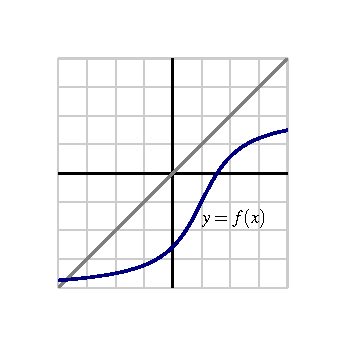
\includegraphics{figures/2_6_Ez4.eps}
\caption{A function $y = f(x)$ for use in Exercise~2.} \label{F:2.6.Ez4}
\end{center}
\end{figure}

\item Consider the graph of $y = f(x)$ provided in Figure~\ref{F:2.6.Ez4} and use it to answer the following questions.
\ba
	\item Use the provided graph to estimate the value of $f'(1)$.
	\item Sketch an approximate graph of $y = f^{-1}(x)$.  Label at least three distinct points on the graph that correspond to three points on the graph of $f$.
	\item Based on your work in (a), what is the value of $(f^{-1})'(-1)$?  Why?
\ea

\item Let $f(x) = \frac{1}{4}x^3 + 4.$
\ba
	\item Sketch a graph of $y = f(x)$ and explain why $f$ is an invertible function.
	\item Let $g$ be the inverse of $f$ and determine a formula for $g$.
	\item Compute $f'(x)$, $g'(x)$, $f'(2)$, and $g'(6)$.  What is the special relationship between $f'(2)$ and $g'(6)$?  Why?
\ea
\item Let $h(x) = x + \sin(x)$.
\ba
	\item Sketch a graph of $y = h(x)$ and explain why $h$ must be invertible.
	\item Explain why it does not appear to be algebraically possible to determine a formula for $h^{-1}$.
	\item Observe that the point $(\frac{\pi}{2}, \frac{\pi}{2} + 1)$ lies on the graph of $y = h(x)$.  Determine the value of $(h^{-1})'(\frac{\pi}{2} + 1)$.
\ea


\end{exercises}
\afterexercises